\documentclass{article}
\usepackage[left=2cm,right=2cm,top=2cm,bottom=2cm]{geometry}
\usepackage[utf8]{inputenc}
\usepackage[german]{babel}
\usepackage{amsmath}
\usepackage{dsfont}
\usepackage[export]{adjustbox}
\usepackage{amsthm}
\usepackage{color}
\usepackage{amsfonts}
\usepackage{amssymb}
\usepackage{wasysym}
\usepackage{makeidx}
\usepackage{graphicx}
\usepackage[colorlinks=true,urlcolor=blue,linkcolor=blue]{hyperref}
\usepackage{ziffer}
\usepackage{minted}
\usepackage{xcolor}
\usepackage{framed}
\usepackage{mdframed}
\usepackage{subfiles}
\usemintedstyle{emacs}

\definecolor{purp}{HTML}{9A72AC}
\definecolor{re}{HTML}{FC6255}
\definecolor{gre}{HTML}{83C167}
\definecolor{blu}{HTML}{58C4DD}
\definecolor{shadecolor}{rgb}{0.85,0.85,0.85}
\definecolor{bg}{rgb}{0.95,0.95,0.95}
\setlength{\parindent}{0em} 

\BeforeBeginEnvironment{minted}{\begin{mdframed}[linewidth =2 ,backgroundcolor=bg , linecolor=black, linewidth=0.5]}
\AfterEndEnvironment{minted}{\end{mdframed}}

\newtheorem{defi}{Definition}
\BeforeBeginEnvironment{defi}{\begin{mdframed}[linewidth =2 ,backgroundcolor=bg , linecolor=black, linewidth=0.5]}
\AfterEndEnvironment{defi}{\end{mdframed}}

\newcommand{\bsp}{\textbf{Beispiel}:}
%\newcommand{\task}{\textbf{Aufgabe}:}

\newcommand{\bol}[1]{\textbf{#1}}
\newcommand{\q}[1]{\glqq #1\grqq}
\newcommand{\DODO}[1]{\textbf{\textcolor{red}{DODO:}} #1 \\ \begin{center}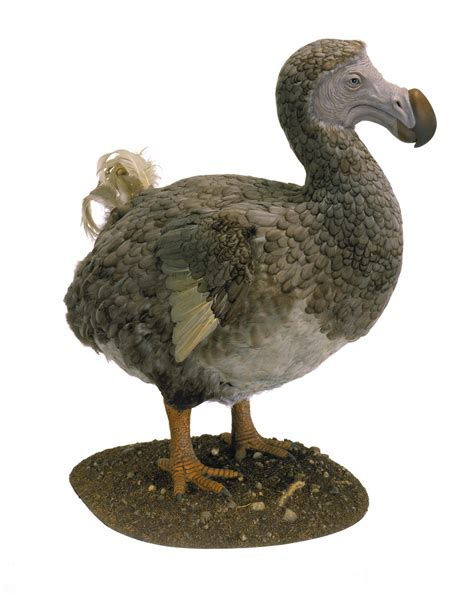
\includegraphics[scale=0.2]{../../media/dodo.jpg} \end{center}}

\newenvironment{task}[1]{
    \begin{shaded*}
    \textbf{Aufgabe #1}:
}{
    \end{shaded*}
}

\begin{document}

Nach diesen Vorüberlegungen und Grundbegriffen können wir uns der Implementierung eines Graphen widmen. Die Struktur der Knoten bzw. der Speicherung von Daten in den Knoten können wir dabei von Bäumen bzw. Listen übernehmen. Das entscheidende neue Element ist also die Repräsentation der Kanten und deren Gewichte. \\

Die beiden häufigsten Möglichkeiten der Implementierung verwenden eine \textbf{Adjazenzmatrix} bzw. \textbf{Adjazenzlisten}, in diesem Kapitel werden wir uns der Matrix widmen. \\
Wir betrachten wieder ein Beispiel aus den Grundlagen:
\begin{center}
    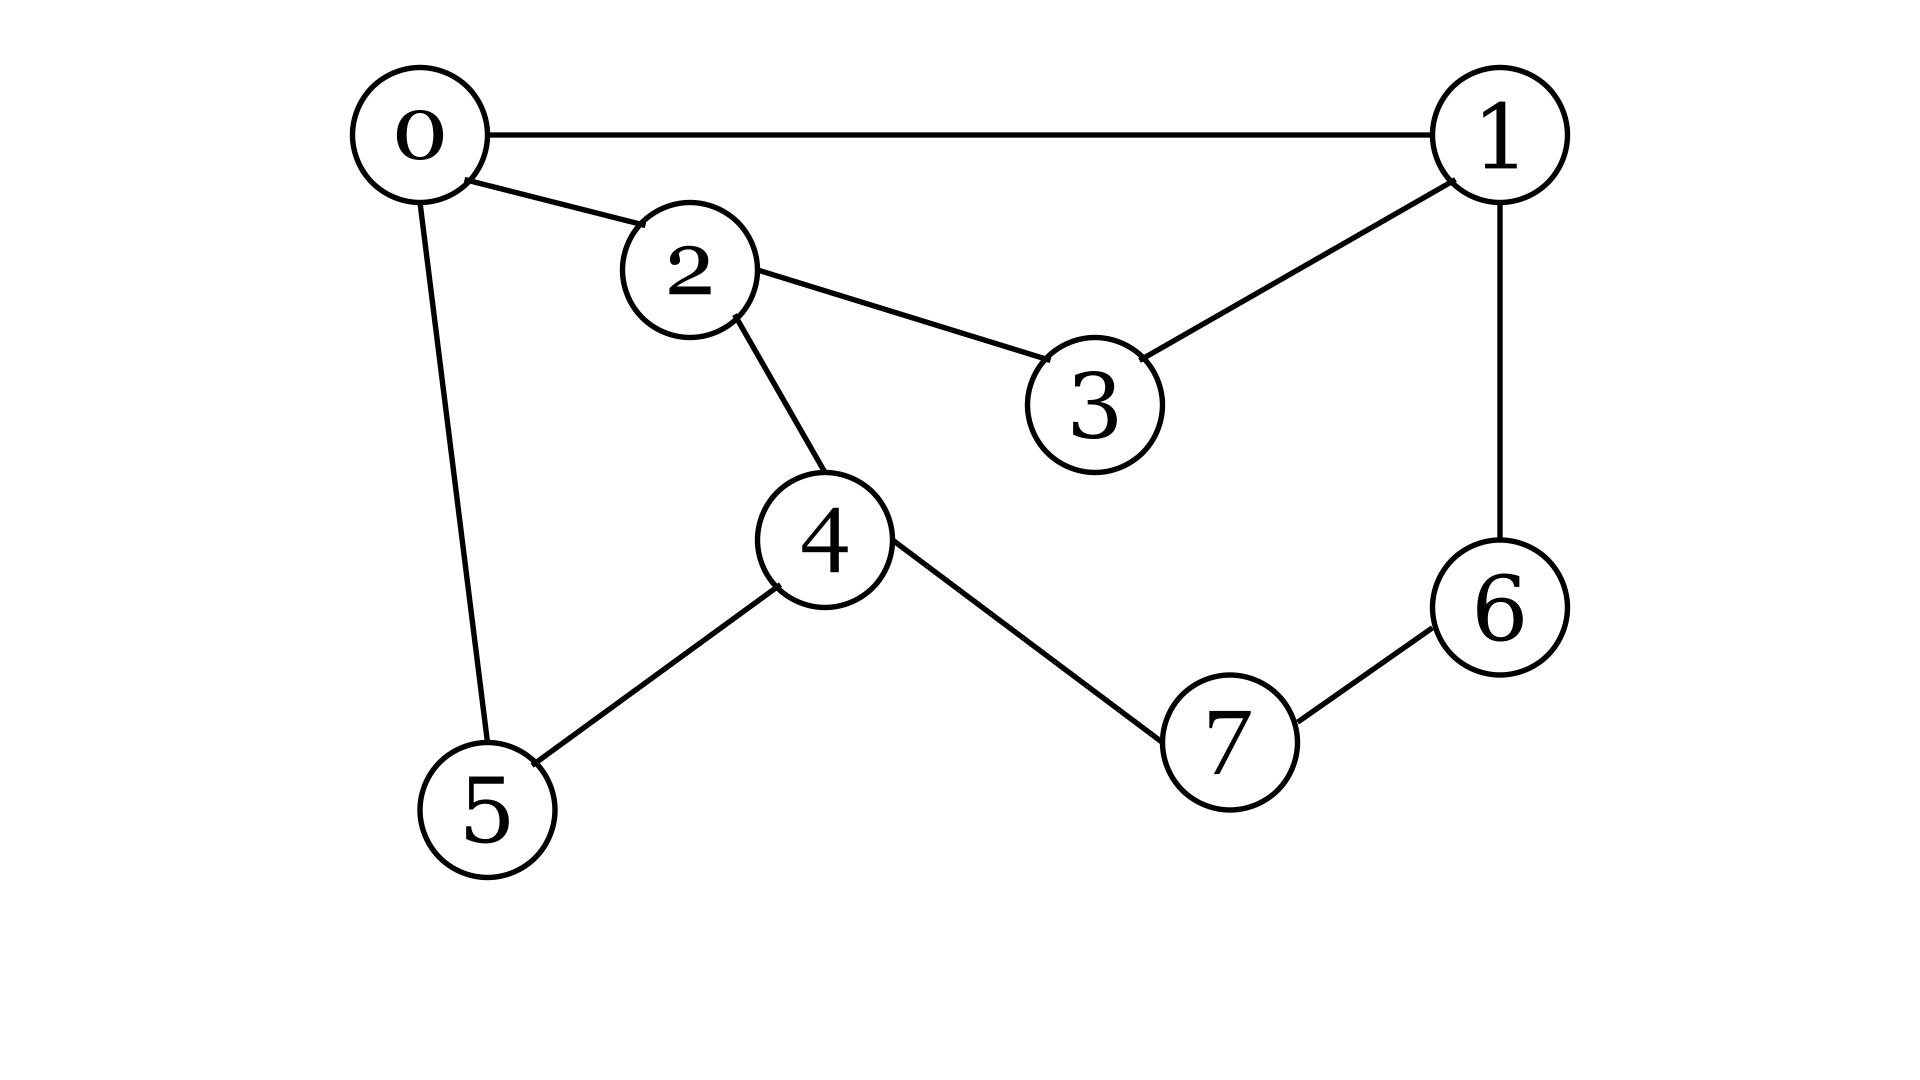
\includegraphics[scale=0.15]{../media/matrix_1.png}
\end{center}
Es handelt sich um einen ungerichteten, zusammenhängenden Graphen. Will man die Verbindungen zwischen den einzelnen Knoten darstellen, bietet es sich an \q{von Knoten zu Knoten} zu denken. Man betrachtet eine Matrix nach folgendem Schema (die einzelnen Knoten werden zusätzlich zu ihrem Index noch mit \textit{k} benannt, um später leichtere Lesbarkeit zu gewährleisten): 
\begin{center}
\begin{tabular}{|c|c|c|c|c|c|c|c|c|}
    \hline 
        & k0 & k1 & k2 & k3 & k4 & k5 & k6 & k7  \\
    \hline 
    k0 & & & & & & & & \\
    \hline 
    k1 & & & & & & & &\\
    \hline 
    k2 & & & & & & & &\\
    \hline 
    k3 & & & & & & & &\\
    \hline 
    k4 & & & & & & & &\\
    \hline 
    k5 & & & & & & & &\\
    \hline 
    k6 & & & & & & & &\\
    \hline 
    k7 & & & & & & & &\\
    \hline 
\end{tabular} 
\end{center}

Wir betrachten exemplarisch die Kante zwischen den Knoten $0$ und $2$. Häufig interpretiert man die Tabelle so, dass auf der linken Seite - also den Zeilen -  die Startknoten abgebildet werden, die Spalten dagegen bilden die Zielknoten. Wollen wir also eintragen, dass eine Kante von $0$ nach $2$ läuft, suchen wir in der Zeile $k0$ die Spalte $k2$ und markieren die entsprechende Zelle: 
\begin{center}
    \begin{tabular}{|c|c|c|c|c|c|c|c|c|}
        \hline 
            & k0 & k1 & k2 & k3 & k4 & k5 & k6 & k7  \\
        \hline 
        k0 & & & \color{red} x \color{black}& & & & & \\
        \hline 
        k1 & & & & & & & &\\
        \hline 
        k2 & & & & & & & &\\
        \hline 
        k3 & & & & & & & &\\
        \hline 
        k4 & & & & & & & &\\
        \hline 
        k5 & & & & & & & &\\
        \hline 
        k6 & & & & & & & &\\
        \hline 
        k7 & & & & & & & &\\
        \hline 
    \end{tabular} 
    \end{center}
Da es sich um einen ungerichteten Graphen handelt, geht aber auch ein Weg von $2$ nach $0$, also muss direkt auch in der Spalte $k0$ und Reihe $k2$ eine Markierung gesetzt werden. \\
Dies wird für alle Einträge der Fall sein! Man spricht hier auch von einer \textbf{symmetrischen} Matrix, d.h. es genügt sich alle Einträge in der \q{oberen rechten Hälfte} anzusehen, d.h. von kleineren zu größeren Zahlen. Danach kann \q{nach unten links} gespiegelt werden. Zunächst tragen wir aber alle weiteren Kanten von kleinerer zu größerer Zahl ein:
\begin{center}
    \begin{tabular}{|c|c|c|c|c|c|c|c|c|}
        \hline 
            & k0 & k1 & k2 & k3 & k4 & k5 & k6 & k7  \\
        \hline 
        k0 & & \color{red} x \color{black}& \color{red} x \color{black}& & & \color{red} x \color{black}& & \\
        \hline 
        k1 & & & &\color{red} x \color{black} & & & \color{red} x \color{black}&\\
        \hline 
        k2 & & & & \color{red} x \color{black}& \color{red} x \color{black}& & &\\
        \hline 
        k3 & & & & & & & &\\
        \hline 
        k4 & & & & & &\color{red} x \color{black} & & \color{red} x \color{black}\\
        \hline 
        k5 & & & & & & & &\\
        \hline 
        k6 & & & & & & & & \color{red} x \color{black}\\
        \hline 
        k7 & & & & & & & &\\
        \hline 
    \end{tabular} 
    \end{center}
Mit den gespiegelten Werten ergibt sich:
\begin{center}
    \begin{tabular}{|c|c|c|c|c|c|c|c|c|}
        \hline 
            & k0 & k1 & k2 & k3 & k4 & k5 & k6 & k7  \\
        \hline 
        k0 & & \color{red} x \color{black}& \color{red} x \color{black}& & & \color{red} x \color{black}& & \\
        \hline 
        k1 & \color{red} x \color{black} & & &\color{red} x \color{black} & & & \color{red} x \color{black}&\\
        \hline 
        k2 &  \color{red} x \color{black} & & & \color{red} x \color{black}& \color{red} x \color{black}& & &\\
        \hline 
        k3 & &\color{red} x \color{black}  & \color{red} x \color{black}  & & & & &\\
        \hline 
        k4 & & & \color{red} x \color{black} & & &\color{red} x \color{black} & & \color{red} x \color{black}\\
        \hline 
        k5 & \color{red} x \color{black} & & & & \color{red} x \color{black}  & & &\\
        \hline 
        k6 & & \color{red} x \color{black} & & & & & & \color{red} x \color{black}\\
        \hline 
        k7 & & & & &\color{red} x \color{black}  & & \color{red} x \color{black}  &\\
        \hline 
    \end{tabular} 
    \end{center}
Jetzt stellt sich die Frage, wie eine solche Matrix in einem Programm darstellen lässt. Die einfachste Variante ist ein zweidimensionales Array. In Bezug auf den Datentyp des Feldes gibt es verschiedene Möglichkeiten. Für einen ungewichteten Graphen ist nur wichtig, ob eine Verbindung zwischen zwei Knoten vorhanden ist, da die Kante keine zusätzlichen Informationen enthält, man könnte hier also ein Boolean-array verwenden, die Tabelle sähe also wie folgt aus:

\begin{center}
    \begin{tabular}{|c|c|c|c|c|c|c|c|c|}
        \hline 
            & k0 & k1 & k2 & k3 & k4 & k5 & k6 & k7  \\
        \hline 
        k0 & \color{red} False \color{black} & \color{green}True\color{black} & \color{green}True\color{black} & \color{red} False \color{black}&\color{red} False \color{black} & \color{green}True\color{black}& \color{red} False \color{black}& \color{red} False \color{black}\\
        \hline 
        k1 & \color{green}True\color{black} & \color{red} False \color{black}& \color{red} False \color{black}&\color{green}True\color{black} &\color{red} False \color{black} & \color{red} False \color{black}& \color{green}True\color{black}&\color{red} False \color{black}\\
        \hline 
        k2 &  \color{green}True\color{black} & \color{red} False \color{black}& \color{red} False \color{black}& \color{green}True\color{black}& \color{green}True\color{black}& \color{red} False \color{black}& \color{red} False \color{black}&\color{red} False \color{black}\\
        \hline 
        k3 & \color{red} False \color{black}&\color{green}True\color{black}  & \color{green}True\color{black}  & \color{red} False \color{black}& \color{red} False \color{black}& \color{red} False \color{black}& \color{red} False \color{black}&\color{red} False \color{black}\\
        \hline 
        k4 &\color{red} False \color{black} & \color{red} False \color{black}& \color{green}True\color{black} & \color{red} False \color{black}& \color{red} False \color{black}&\color{green}True\color{black} & \color{red} False \color{black}& \color{green}True\color{black}\\
        \hline 
        k5 & \color{green}True\color{black} & \color{red} False \color{black}& \color{red} False \color{black}&\color{red} False \color{black} & \color{green}True\color{black}  & \color{red} False \color{black}& \color{red} False \color{black}&\color{red} False \color{black}\\
        \hline 
        k6 &\color{red} False \color{black} & \color{green}True\color{black} & \color{red} False \color{black}& \color{red} False \color{black}& \color{red} False \color{black}& \color{red} False \color{black}&\color{red} False \color{black} & \color{green}True\color{black}\\
        \hline 
        k7 & \color{red} False \color{black}& \color{red} False \color{black}&\color{red} False \color{black} &\color{red} False \color{black} &\color{green}True\color{black}  & \color{red} False \color{black}& \color{green}True\color{black}  &\color{red} False \color{black}\\
        \hline 
    \end{tabular} 
    \end{center}
Sobald allerdings Kantengewichte eine Rolle spielen, ist ein boolean-array nicht mehr ausreichend, da die Gewichte nicht mehr anderweitig gespeichert werden sollten. Geht man davon aus, dass sich alle Informationen, die man codieren möchte in irgendeiner Form durch Zahlen ausdrücken lassen, so wäre ein \textbf{double[ ][ ]}-array geeignet, um möglichst viele Spielarten von Graphentypen abbilden zu können. In unserem Fall ohne Gewichte könnte dann beispielsweise $1$ für \q{Kante existiert} und $0$ für \q{Kante existiert nicht} stehen: 

\begin{center}
    \begin{tabular}{|c|c|c|c|c|c|c|c|c|}
        \hline 
            & k0 & k1 & k2 & k3 & k4 & k5 & k6 & k7  \\
        \hline 
        k0 & \color{red} 0 & \color{green} 1 & \color{green} 1 & \color{red} 0&\color{red} 0 & \color{green} 1& \color{red} 0& \color{red} 0\\
        \hline 
        k1 & \color{green} 1 & \color{red} 0& \color{red} 0&\color{green} 1 &\color{red} 0 & \color{red} 0& \color{green} 1&\color{red} 0\\
        \hline 
        k2 &  \color{green} 1 & \color{red} 0& \color{red} 0& \color{green} 1& \color{green} 1& \color{red} 0& \color{red} 0&\color{red} 0\\
        \hline 
        k3 & \color{red} 0&\color{green} 1  & \color{green} 1  & \color{red} 0& \color{red} 0& \color{red} 0& \color{red} 0&\color{red} 0\\
        \hline 
        k4 &\color{red} 0 & \color{red} 0& \color{green} 1 & \color{red} 0& \color{red} 0&\color{green} 1 & \color{red} 0& \color{green} 1\\
        \hline 
        k5 & \color{green} 1 & \color{red} 0& \color{red} 0&\color{red} 0 & \color{green} 1  & \color{red} 0& \color{red} 0&\color{red} 0\\
        \hline 
        k6 &\color{red} 0 & \color{green} 1 & \color{red} 0& \color{red} 0& \color{red} 0& \color{red} 0&\color{red} 0 & \color{green} 1\\
        \hline 
        k7 & \color{red} 0& \color{red} 0&\color{red} 0 &\color{red} 0 &\color{green} 1  & \color{red} 0& \color{green} 1  &\color{red} 0 \color{black}\\
        \hline 
    \end{tabular} 
    \end{center}
Alternativ könnte auch z.B. $-1$ und $1$ oder jede beliebige andere Kombination verwendet werden. \\
Diese Implementierung hat natürlich den Nachteil, das bei vielen Knoten, aber wenigen Kanten viele Einträge in der Matrix gleich $0$ sind. Man spricht von einer \q{dünn besetzten Matrix}. Für unsere kleinen Graphen ist das nicht so schlimm, aber möchte man beispielsweise das Straßennetz einer Stadt - oder von ganz Deutschland, oder der Welt! - modellieren, stellt das einen unnötigen Verbrauch von Speicherplatz dar. In der \q{Realität} wird häufig die Idee der Adjazenmatrix beibehalten, aber die Speicherung der Information wird auf andere Datenstrukturen als ein $n\cdot n$ - Feld ausgelagert (mit $n$ der Anzahl der Knoten!). Verwendet werden z.B.:
\begin{itemize}
    \item \textbf{Dictionarys} (DOK: Dictionary of keys: in Java z.B. HashTables, HashMaps): Es werden (Zeile, Spalte)-Paare auf den Kantenwert abgebildet.
    \item \textbf{Coordinate list}: es werden direkt (Zeile, Spalte, Kantenwert)-Tripel gespeichert. 
    \item \textbf{Compressed sparse row} (Yale format): Es werden drei Arrays gespeichert: eines für die Kantenwerte, eines für die Spaltenindizes an denen diese stehen und eines für die Zeilenindices.
\end{itemize}
In allen drei Fällen werden die Null-Werte nicht mehr mitgespeichert, aber zurück zu unserer - deutlich einfacheren - Implementierung. Ein mögliches Klassendiagramm für unseren Graphen sieht wie folgt aus: 
\begin{center}
    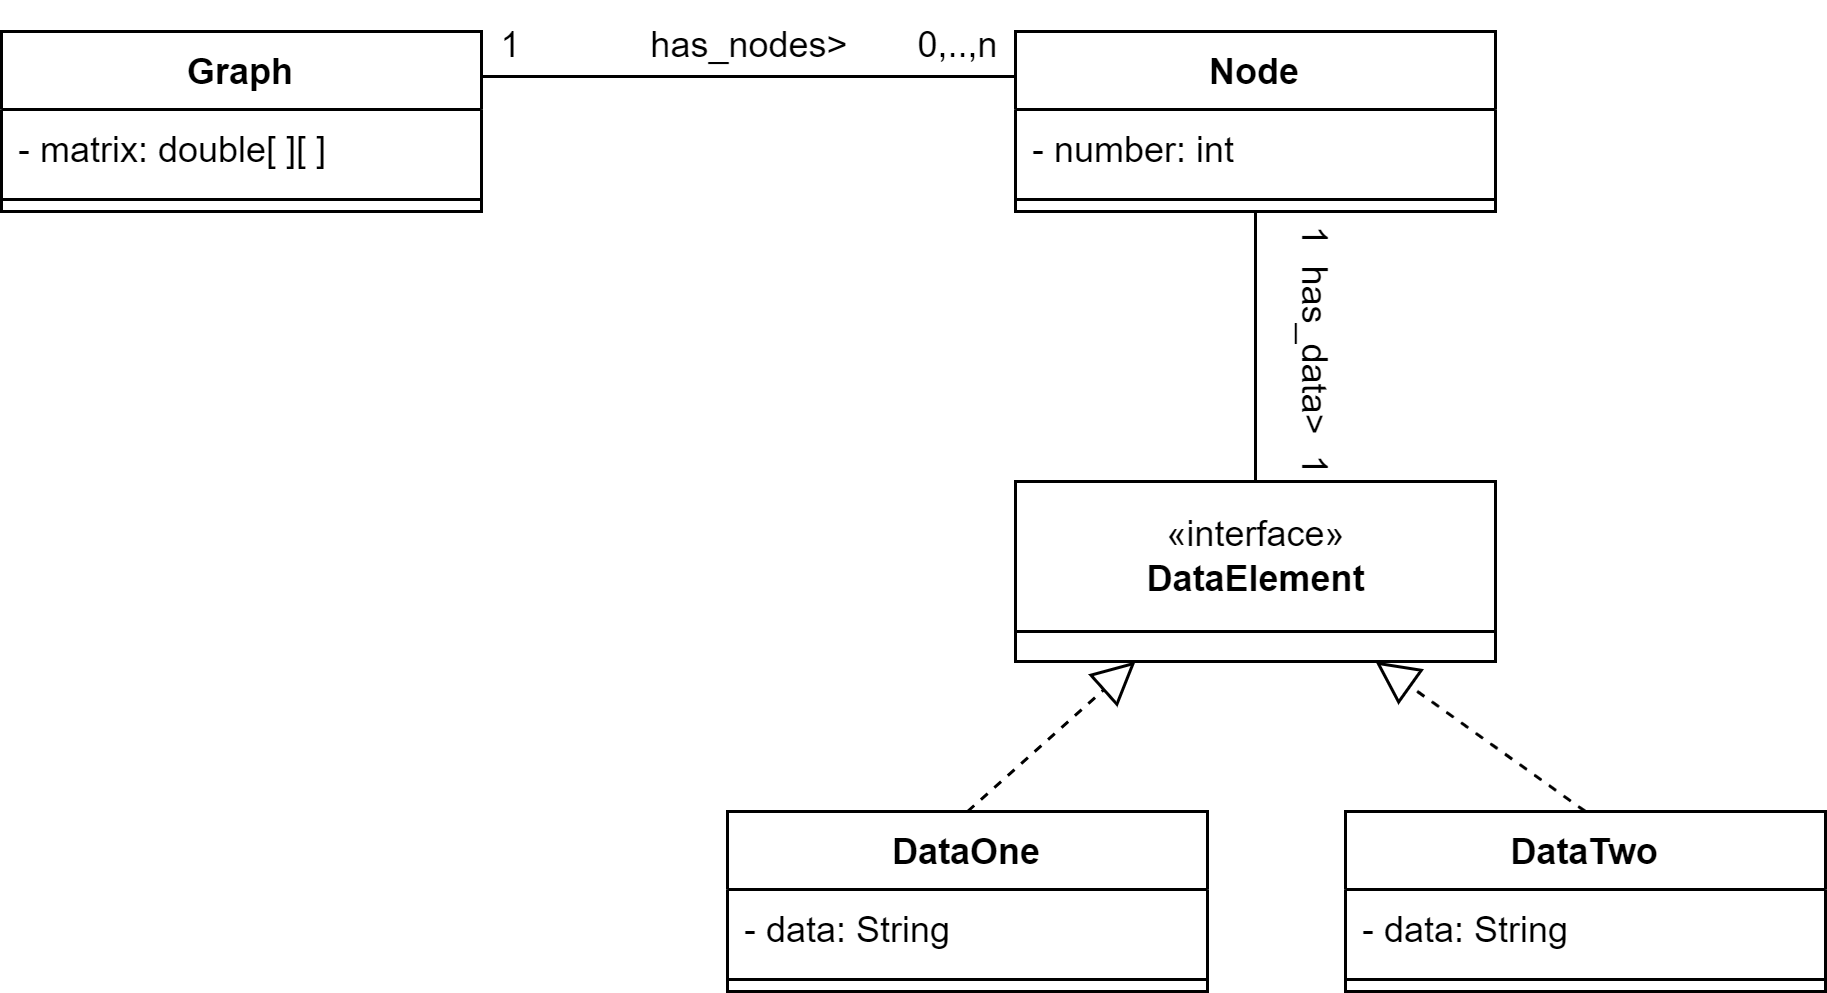
\includegraphics[scale=0.2]{../media/graph_advanced.png}
\end{center}
Das Attribut \textbf{maxNodes} ist nicht zwingend notwendig, es hängt davon ab, ob man den Graphen erweiterbar gestalten möchte oder nicht. Der Vorteil der Verwendung eines Maximums besteht darin, dass das zweidimensionale Feld direkt mit seiner endgültigen Größe erzeugt werden kann. Ansonsten müsste beim Hinzufügen eines Knotens immer die Adjazenzmatrix vergrößert werden, was nur durch Erzeugen eines neuen Arrays und Kopieren des Alten Arrays möglich wäre. \\
Im Folgenden wollen wir uns außerdem darauf beschränken, dass die Knoten des Graphen keine weiteren Informationen verwalten müssen außer ihrer eigenen Nummer. Wir wollen außerdem bei Erstellung des Graphen festlegen, wie groß er ist, da dies der Regelfall im Einsatz ist, d.h. ein grundlegendes Klassendiagramm unseres einfachstmöglichen Graphen sieht (noch ohne Methoden) wie folgt aus: 
\begin{center}
    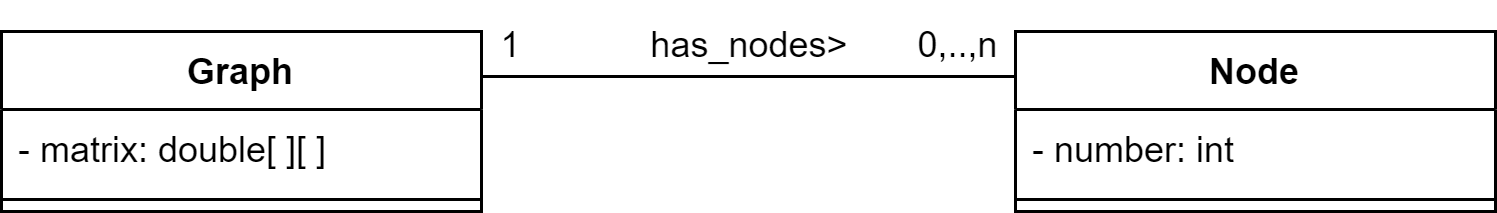
\includegraphics[scale=0.2]{../media/graph_basic.png}
\end{center}
\begin{task}{1}
Implementieren Sie die Grundstruktur des Graphen mit Adjazenzmatrix nach obigem vereinfachten Klassendiagramm, zusätzlich soll es folgendes geben: 
\begin{itemize}
    \item einen Konstruktor, der einen Graphen mit einer bestimmten Anzahl an Knoten erzeugt. 
    \item einen Konstrukter, der einen Graphen erzeugt, wenn eine Knotenliste und eine Adjazenzmatrix übergeben werden.
    \item eine Methode, die eine Kante ohne Gewicht hinzufügt.
    \item eine Methode, die eine Kante mit Gewicht hinzufügt.
    \item für die beiden vorangehenden Methoden jeweils eine Methode, die außerdem die \q{Rückrichtung} gleich mit setzt (für ungerichtete Graphen).
    \item eine Methode, die einen Knoten hinzufügt, wenn die Maximalzahl noch nicht erreicht ist.
    \item eine Methode, die prüft, ob zwischen zwei Knoten eine Kante existiert.
    \item eine Methode, die eine existierende Kante löscht und eine Option, die eine Kante in beide Richtungen löscht!.
    \item eine Methode, die die Adjazenzmatrix lesbar auf der Konsole ausgibt. 
\end{itemize}
\end{task}
Die Lösung zu dieser Aufgabe findet sich auf der nächsten Seite.


\newpage

Wir beginnen mit der Knoten-Klasse, hier gibt es aktuell noch nicht viel zu tun:
\begin{minted}{java}
public class Node {

    private int number;

    public Node(int number) {
        this.number = number;
    }
}
\end{minted}
In der Graphen-Klasse sind die Konstruktoren zuerst an der Reihe: 
\begin{minted}{java}
public class Graph {

    private double[][] matrix;
    private Node[] nodes;

    public Graph(double[][] matrix, Node[] nodes) {
        this.nodes = nodes;
        this.matrix = matrix;
    }


    public Graph(int nodeNumber) {
        if(nodeNumber <= 0) nodeNumber = 5;
        nodes = new Node[nodeNumber];
        for(int i = 0; i < nodeNumber; i++) {
            nodes[i] = new Node(i);
        }
        matrix = new double[nodeNumber][nodeNumber];
    }
}
\end{minted}
Im zweiten Fall werden die Knoten von $0$ bis $nodeNumber - 1$ erzeugt und im Knoten-Array gespeichert. Wir können ein Array verwenden, da wir davon ausgehen, dass sich die Größe unseres Graphen nicht mehr verändert. Ansonsten könnten wir natürlich auch eine Liste verwenden! \vspace{2mm} \\

Die Methoden um die Kanten hinzuzufügen sind vergleichsweise simpel: es muss jeweils in der Matrix an der korrekten Stelle entweder eine $1$ platziert werden, oder der Wert des übergebenen Gewichts für diese Kante. Damit ergeben sich die folgenden vier Methoden (jeweils noch eine zusätzlich, um gleich beide Kanten für einen ungerichteten Graphen zu erzeugen). Die vorangestellte checkInput()-Methode wird dazu verwendet, in jedem Fall zu prüfen, ob die übergebenen Indices zu unserem Knotenarray passen:
\begin{minted}{java}
public boolean checkInput(int start, int end) {
    if(start < 0 || end < 0 || start > nodes.length || end > nodes.length) {
        System.out.println("There cannot be an edge here!");
        return false;
    }
    return true;
}

public void addEdge(int start, int end) {
    if(checkInput(start, end)) matrix[start][end] = 1;
}

public void addEdge(int start, int end, double weight) {
    if(checkInput(start, end)) matrix[start][end] = weight;
}

public void addEdgeBoth(int start, int end) {
    if(checkInput(start, end)) {
    matrix[start][end] = 1;
    matrix[end][start] = 1;
    }
}

public void addEdgeBoth(int start, int end, double weight) {
    if(checkInput(start, end)) {
        matrix[start][end] = weight;
        matrix[end][start] = weight;
    }
}
\end{minted}
Wir gehen hier davon aus, dass die einzige relevante Information eines Knotens seine Nummer ist, mit der wir ihn erzeugt haben. Da diese Nummer auch der Position im Array entspricht (deswegen der Beginn bei 0), können wir den Methoden hier direkt die Positionen im Array übergeben, um die Kanten zu definieren. Möchte man sich nicht auf diese Reihenfolge verlassen bzw. sie benutzen, so muss jeder Knoten mit einem anderen Attribut eindeutig zuordbar sein. Dann kann jeweils dieses Attribut der \textit{addEdge()} - Methode übergeben werden und die entsprechenden Knoten können im Array gesucht werden. \\
Bei der Methode, die prüft, ob eine Kante existiert, gibt es nicht viel zu beachten, ebensowenig bei den Methoden zum Löschen:
\begin{minted}{java}
public boolean existsEdge(int start, int end) {
    if(!checkInput(start, end)) return false;
    if(matrix[start][end] != 0) {
        return true;
    }
    return false;
}

public void removeEdge(int start, int end) {
    if(checkInput(start, end)) matrix[start][end] = 0;
}

public void removeEdgeBoth(int start, int end) {
    if(checkInput(start, end)) {
        matrix[start][end] = 0;
        matrix[end][start] = 0;
    }
}
\end{minted}
Die Ausgabe-Methode schreibt zusätzlich zu den Gewichten noch die Knotennamen in die oberste Spalte bzw. Zeile. Der Tabstop wird verwendet, damit die Zahlen hübscher untereinander angezeigt werden. 
\begin{minted}{java}
public void printMatrix() {
    System.out.print("\t");
    for(int i = 0; i < nodes.length; i++) {
        System.out.print("k" + i + "\t");
    }
    for(int i = 0; i < nodes.length; i++) {
        System.out.println();
        System.out.print("k" + i + "\t");
        for(int j = 0; j < nodes.length; j++) {
            System.out.print(matrix[i][j] + "\t");
        }
    }
}
\end{minted}

Alle weiteren möglicherweise interessanten Methoden, werden wir in Kapitel 4 - Graphenalgorithmen - implementieren. 
\end{document}